\chapter{Materials and Methods}

\section{Magnetic Sensor Device} 
\todo{Foto of setup with arrows to necessary parts	Microscope	Stages	PEEK holder	Helmholtz coils	Kepco MFLI	DAQ	Loss because of reduced velocity and magnetic drag Different produced GMR stacks	Wheatstone Bridge setup	Magnet alignment}
\subsection{Assembly of Sensor}
\label{sec:meth:sensor}
The fabrication of a microfluidic device on various substrates and layouts consists of two parallelizable workflows. First, the \gls{gmr}-sensor chip (Sensitec) is assembled into a custom designed PCB (Piu-Printex) by double sided adhesive tape and a square glass slide (\SI{25}{\milli\meter}x\SI{25}{\milli\meter}, Thermo Scientific) at the bottom. A connection in between was formed by wedge wire bonding (HB10, TPT) which bonded \SI{25}{\micro\meter} thick gold wire to the respective gold bond pads. The optimal parameters are listed in table \ref{tab:params_wirebonding}. 
\begin{table}[htb]
	\centering
\begin{tabularx}{.5\linewidth}{ccc}
	\toprule[1pt]
	Parameters & Bond 1 & Bond 2 \\
	\midrule
	Ultrasonic Power & 250 & 300 \\
	Time / ms & 200 & 200 \\
	Force / mN & 250 & 300 \\
	\bottomrule[1.2pt]
\end{tabularx}
\caption{Wirebonding Parameters}
\label{tab:params_wirebonding}
\end{table}
However, crucial for successful wire bonding is the optimal hole shape in the welding tool. Therefore, it was cleaned when bonds failed for no obvious reason by removing the gold wire and dipping the tip of the wedge into \gls{ipa}. Then, \textit{Test USG} was alternated for several seconds in multiple iterations. Afterwards, the wedge was blown dry from all sides with pressurized air and the wire was loaded back into the tool.
After wire bonding, the manufactured sensors were placed in a wafer shipper box and stored in a dust free environment upon further use.

\subsection{Design and Fabrication of Microfluidics}
In the second workflow, a microfluidic channel was manufactured via photo- and softlithography and bonded to the produced sensors from \ref{sec:meth:sensor}.
\subsubsection{Development of Layout}
\todo{layout design, hier noch die mänder und verengungen oder den kaptten 150u wafer?}

\subsubsection{Patterning of Photoresist}
\SI{3}{\inch} (100) silicon wafers (Si-Mat) were dehumidified in a drying oven (UN30, Memmert) for \SI{2}{\hour} at \SIrange{150}{180}{\degreeCelsius}. Then, immediately after they reached room temperature, they were placed centered inside a wafer spinner (WS-650-23B, Laurell Technologies). For the desired layer thicknesses \SIrange{2}{3}{\milli\liter} SU8-30XX (Microchem) were poured carefully onto the center of the wafer and the following program was carried out:
\begin{enumerate}[noitemsep]
\item \SI{500}{\rpm} for \SI{10}{s} at \SI{100}{\rpm\per\second}
\item \SI{3000}{\rpm} for \SI{30}{s} at \SI{300}{\rpm\per\second}
\item Ramp down at \SI{300}{\rpm\per\second}
\end{enumerate}
Upon finish, the wafer was gripped outermost with wafer tweezers and soft-baked on a hot plate (super nuova+, Thermo Scientific) for \SI{5}{\minute} at \SI{65}{\degreeCelsius} and at least \SI{10}{\minute} at \SI{90}{\degreeCelsius}. The optimal duration was determined if the gently touched resist did not stick to the tweezers. To prevent cracks in the resist caused by a fast temperature change, the wafer was cooled on the hotplate to room	temperature. Such processed wafers were stored for a maximum of \SI{4}{weeks} in a light-tight storage box.\\
To pattern the resist, the i-Line of a laser lithograph (Dilase 250, Kloe) was used. In preparation of the writing layout a AutoCADz \textit{*.dxf}-file with only one layer of polylines was imported to the program ``Kloe Design'', converted to contours and subsequently to polygons. For the filling a spot-size equivalent to the minimal structure resolution (as measured in \citet{lit:tech:rojda2020}) and an overlap of at least \SI{50}{\percent} was chosen. Departure and End Stabilization were chosen to \SI{.5}{\milli\meter} in a horizontal infill pattern. Also, flags for \textit{auto-reverse mode}, \textit{apply multiple trigger}, and \textit{detect partial/full overlap} have been set.  The writing trajectories were displayed for a last control before the export to ensure only closed contours. Finally the contour and filling were exported into separate files.\\
Both files were loaded in this order into the program ``Dilase 250''. Also the preprocessed wafer was placed inside the laser writer and attached to the vacuumed stage. With the integrated camera the global zero was set to the wafer center by finding the horizontal or vertical edges and adding/subtracting the radius of the wafer (\SI{1.5}{\inch} $\approx\ \varnothing $  \SI{38.1}{\milli\meter}). The focus point was set to the top of the resist and subsequently moved \SI{.07}{\milli\meter} relative down for thick layers. Then the program was initiated with \SI{100}{\percent} laser modulation and \SIrange{20}{40}{\milli\meter\per\second} writing velocity.

\subsubsection{Soft Lithography}
The fabricated wafer was placed the center of a \SI{90}{\centi\meter} petri dish. A \gls{pdms} mold was created by vigorous mixing of the pre-polymer base with its curing agent (Sylgard 184, Dowsil) in a ratio of 10:1 (w/w). For \SI{3}{\inch} wafers, thin channels were casted from \SI{15}{\gram}, normal channels from \SI{20}{\gram} PDMS in the petri dish. Gas bubbles were removed from the mixture in a desiccator for \SI{20}{\minute} at \SI{2}{\hecto\pascal} , and the clear \gls{pdms} was cured in an oven (Um, Memmert) for \SI{1}{\hour} at \SI{60}{\degreeCelsius}. After curing, the \gls{pdms} mold was released from the petri dish carefully, taken off the wafer and stored in a clean petri dish upon further processing.  

\subsubsection{Bonding of Microfluidics}
Under laminar flow, crosslinked molds were cut into pieces with the respecting single \gls{uf} with a razor blade. Holes for in- and outlet were punched through the containing channels with a biopsy puncher (ID \SI{0.5}{\milli\meter}, WellTech). The substrates and \glspl{uf} were sonicated in acetone and \gls{dih2o} for \SI{5}{\minute} and dried with filtered \gls{n2} completely. For the bonding of PDMS to various substrates different protocols have been established:

\subsubsection{PDMS Glueing}
\label{sec:meth:bond:glue}
Here, a micron-height layer of uncured \gls{pdms} was used as an adhesive layer between \gls{uf} and substrate. Approx. \SI{3}{\milli\liter} were poured onto a \SI{3}{\inch} wafer and spun down for \SI{5}{\minute} at \SI{6000}{\per\minute}. The microchannel was placed on the substrate by visual control of a stereo microscope (SMZ800, Nikon) with 8-fold magnification. Subsequently, the bonding process could be finished by a \SI{1}{\hour} bake at \SI{60}{\degreeCelsius} or over-night at room temperature.
\subsubsection{Plasma Bonding}
\label{sec:meth:bond:plasma}
The respective parts were activated by the exposure to a controlled \gls{o2}-plasma. Bringing the activated surfaces in contact immediately triggers the formation of covalent bonds. First, the acetone-wiped substrates and the microchannels were centered inside the plasma cleaner (Zepto, Diener). Second, vacuum was applied to a final pressure <\SI{0.2}{\hecto\pascal}. Third, the chamber was flushed with pure \gls{o2} until a chamber pressure from \SIrange{0.6}{0.8}{\hecto\pascal} had been stabilized. Fourth, the plasma process was executed with \SI{30}{\watt} (Power-Potentiometer: 100) for \SIrange{45}{60}{\second} (Time-Potentiometer: 15-20). Upon finish, the chamber was flushed for \SI{5}{\second} and ventilated. Immediately after, the corresponding workpieces were brought into contact and pressed together gently. To ensure a durable bond, the assembled structures were baked for \SI{1}{\hour} at \SI{60}{\degreeCelsius}.

\todo{Mass flow equation}

%\begin{equation}
%	Here goes the mass flow equation
%\end{equation}

\subsubsection{Reversible Bonding}
To bond the \gls{uf} to a substrate reversibly and without residues, the channel can be brought into contact with the bottom part without any adhesinon agent. For low-pressure as well as vacuum driven flows, this method is preferrable due to its time and work efficiency.

\subsection{Peripheral Components and Optical Readout}
Each sensor chip was characterized by the hysteresis steepness (equivalent to the sensitivity) and the zero-crossing at half-maximum in a customized setup. Therefore, the underlying 32 x 27 x \SI{5}{\milli\meter} NeFeB magnet (NE3227, IBS Magnet) was adjusted on micromanipulator tables (PT, Thorlabs) in three axes to optimize both parameters. Afterwards, PTFE-tubing (ID \SI{0.5}{\milli\meter}, Reichelt Chemietechnik) was connected on the in- and outlet of the microfluidic. A dispensing tip (OD \SI{0.42}{\milli\meter}, Nordson) was connected to the inlet tubing. Initially a \SI{1}{\milli\liter} syringe (ID \SI{4.72}{\milli\meter}, Terumo) was connected with \gls{dih2o} or \gls{pbs} and flushed with \SIrange{100}{200}{\micro\liter\per\minute} by a syringe pump (Fusion 4000, Chemyx).
\subsubsection{Hysteresis Alignment}
For any used \gls{gmr}-sensor, a characterization of its sensitivity (\si{\volt\per\tesla})  was performed. Therefore, its hysteresis was imposed by two Helmholtz coils ($L_s$ = \SI{167}{\milli\henry}, d = \SI{150}{\milli\meter}, Brockhaus) generating \SI{7.8}{\milli\tesla\per\ampere} orthogonal to the easy axis of the GMR which were driven by a voltage-controlled current source (BOP 50-8M, Kepco Inc.) with $\pm$ \SI{2}{\ampere} at a \gls{el:vpp} of \SI{20}{\volt}. The control voltage was supplied by LabView (2018, 32-bit, National Instruments) supplied by a digital I/O card (USB-6351, National Instruments) in the range of \SIrange{-10}{10}{\volt}.
The resulting sensor signal was fed into the current input of a lock-in amplifier ( \gls{mfli}, \SI{5}{\mega\hertz}, Zurich Instruments). %@@@ Parameters of this
Redigitization and processing was carried out by the same digital I/O card and labview program as for the input control.
\subsubsection{Single GMR} \label{sec:meth:singleGMR}
The change in resistivity over one whole Wheatstone bridge was measured with a fully-integrated lock-in amplifier ( \gls{mfli}, \SI{5}{\mega\hertz}, Zurich Instruments) by a reference \gls{el:vp} of \SIrange{100}{800}{\milli\volt}. The reference frequency was chosen randomly in a range of \SI{100(25)}{\kHz} such that any harmonics were avoided. The measured differential bridge balance was then demodulated and filtered with a time constant of \SI{299.7}{\micro\second} by a third order low-pass filter and amplified by the factor \num{10000}. Subsequently, the processed signal was sampled at \SI{53.2}{\kilo\siemens\per\second}, fed into a digital I/O device (USB-6351, National Instruments) with input range \SIrange{-10}{10}{\volt} and processed in LabView.\newline
Additionally, a 40x microscope image (DM2500, Leica Microsystems) was captured by a CCD-camera (Grasshopper3, FLIR) and displayed in real-time to control the experiment.
\subsubsection{Dual GMR}
\label{sec:meth:dualGMR}
For the measurement of two GMR-sensors simulataneously, the setup from \ref{sec:meth:singleGMR} was duplicated in two different manners. However, the exact same settings in the device control software were crucial for successful measurements.  In a first approach, the supply cable of one \gls{mfli} was splitted and fed into both sensors, while the bridge balance was evaluated by the same and an additional lock-in, both with the exact same settings. Consequently, the ground pin of the one sensor was the reference also for the other sensor and one ground pin was therefore left floating. This method posed the least cable length and therefore noise, but was also prone to cross-talking between the used BNC-cables respectively -connectors. \todo{circuit/picture of both?}

Second, two \gls{mfli}'s were driven in a master-slave clock synchronization by the Multi-Device Sync function. Therefore, the \textit{trigger out} and \textit{clock out} ports on the backside of the master were connected to the slave's \textit{trigger in} and \textit{clock in} ports. Additionally, the \textit{trigger out} was split by a T-connector piece in order to feed it also back into the master's \textit{trigger in} port.

In both cases, the output of both lock-ins was directed to their respective \textit{AUX 1} ports and connected to another LabView program by the previously mentioned DAQ-card.

\subsubsection{Differential Sensor Setup}
In some experiments, two PCBs were stacked with nylon spacers (\todo{spacers}) with various spacings \SIlist{3;5;8}{\milli\meter} between their edges above the permanent magnet. Additionally the outlet tubing of the upper chip was connected to the inlet of the lower chip with the least dead volume possible. The hysteresis was then adjusted for both sensors on various bridges consecutively. Measurements were performed as described in \ref{sec:meth:singleGMR} with two completely independent lock-in amplifiers.

\begin{figure}[h!]
	\includegraphics[width=.5\linewidth]{example-image} 
	\caption{Here comes a nice drawing from the stacked pcb setup}
\end{figure}

\subsubsection{GMR Data Analysis} \label{sec:meth:gmrDataAnalysis}
Subsequent data analysis of the acquired streams from both two and one sensor measurements were modified by a custom labview VI to cut the first sample of the stream which was mandatory for the next step. Next, the characteristic signal patterns were detected in the continuous stream by the \textit{GMR\_Tool\_227} by a rolling-mean thresholding method. The resulting \textit{*\_ana.csv} files were then processed by a custom Matlab script, which in turn computed averages and simple parameters of a single detected signal or whole measured, p.e. the total volume or the signal count therein. The Matlab script saved any analyzed data also in the *.csv format which was finally plotted in Origin (2020b, OriginLab)\todo{maybe block diagram for workflow?}

\section{Magnetic Beadometry}
Magnetic beads were measured in various manners. First, beads were let rolling over functionalized substrates under microscope control (DM6, Leica) and image acquisition for count and trajectory analyses (LAS X, Leica). Second, beads were measured in buffer in whole blood samples magnetically to determine their concentration in the different samples. The previous concentration measurements were then adapted to functionalized surfaces in order to detect a difference in concentration. In all experiments, PTFE-tubing (ID \SI{0.5}{\milli\meter}, Reichelt Chemietechnik), dispensing tips (OD \SI{0.42}{\milli\meter}, Nordson), \SI{1}{\milli\liter} syringes (ID \SI{4.78}{\milli\meter}, Terumo), a syringe pump (Fusion 4000, Chemyx) and a microfluidic channel with dimension \SI{700}{\micro\meter} x \SI{150}{\micro\meter} (width x height) were used.
%\subsection{Optical Particle Tracking}

%\subsection{Absolute Concentration Measurements}

\todo{Concentration Measurement}

\todo{Whole Blood Bead Spiking}

\subsection{Bead Capture Assay}
As prequisite for the bead capture assay, the concentration of different self-biotinylated particles was determined meticulously in a Neubauer Improved counting chamber as well as by flow cytometry and adjusted between \SIrange{1}{10}{\per\micro\liter} in \gls{pbst}. Further, a GMR sensor was fabricated, loaded unspecifically with \SI{1}{\milli\gram\per\milli\liter} neutravidin, hysteresis aligned and connected in the single GMR setup (see \ref{sec:meth:singleGMR}). As first step, the bead adhesion was determined by finding the minimal flow rate at which non-biotinylated beads were still rolling freely and at second, by finding the maximal flow rate at which biotinylated beads were still notably captured, both by microscope oberservation and sensor signal analysis. The average flow rate of these two was consequently held constant over all experiments. Subsequently, beads with different surface coverages of biotin were pumped alternatingly through the channel and over the sensor. The generated data was analyzed after the standard protocol in \ref{sec:meth:gmrDataAnalysis}.

\section{Surface Bio-Functionalization}
\subsection{Surface Activation}
\label{sec:meth:surfActiv}
To functionalize any silicon containing surface with \ch{Si\bond{sb}OH} groups which the utilized silane could interact with, multiple surface activation pathways were explored. First, substrates were cleaned in \gls{hcl}:\gls{meoh} and \gls{h2so4} before they were immersed in boiling water. Second, surface silanol groups were achieved by piranha immersion. Third a \gls{hf} dip and fourth a oxygen plasma treatment was tested.\\
For all methods, the following reagents were used: \gls{dih2o} (\SI{0,054}{\micro\siemens}, Merck MilliQ)), acetone (\SI{>99,9}{\percent}, VWR), \gls{etoh} (absolute, VWR), \gls{meoh} (\SI{99.8}{\percent}, VWR), \gls{acoh} (glacial, VWR), \gls{hcl} (\SI{37}{\percent}, Sigma-Aldrich), \gls{h2so4} (\SIrange{95}{98}{\percent}, VWR), \gls{h2o2} (\SI{30}{\percent} (w/w), Sigma-Aldrich), \gls{hf} (\SI{10}{\percent}, VWR)

\subsubsection{Work Safety Remarks}
Before the work with one of the acid solutions was carried out, serveral safety measures were implemented. As any reacting acid solution becomes very hot immediately due to the exothermic reaction, every container should be placed inside a cooled water or ice bath. Additionally, the beaker as well as concentrated acid flasks should be gripped firmly by a laboratory stand to avoid a tip over. As the reactivity of chemicals is highly temperature-dependent, the solutions was processed further when they had been cooled to \SI{<=80}{\degreeCelsius}. It should be also noted that - as in every chemical reaction, but especially ones with \gls{h2so4} and \gls{hf} - the acid was always poured into the other reactant to avoid splashing and boiling.

\subsubsection{Plasma Activation}
For the plasma activation, process parameters similar to the PDMS bonding technique in \ref{sec:meth:bonding:plasma} were chosen. After inital cleaning via sonication in \gls{acoh} and \gls{dih2o} for \SI{5}{\minute} each, the substrated were dried in \gls{n2}-gas and placed inside the plasma chamber. The chamber was evacuated to a final pressure <\SI{0.2}{\hecto\pascal} and then flushed with pure \gls{o2} until a chamber pressure between \SIrange{0.6}{0.8}{\hecto\pascal} had been stabilized. Fourth, the plasma process was executed with \SI{100}{\watt} (Power-Potentiometer: 300) for \SI{300}{\second} (Time-Potentiometer: \todo{time poti for hydrophobic surface}
). Upon finish, the chamber was flushed for \SI{5}{\second} and ventilated.

\subsubsection{Hydrochloric-Sulfuric Acid Activation}
In order to degrease any glass or \gls{sin} surface, a protocol according to \citet{lit:chem:Dressick} was used. There, the surfaces were first sonicated in acetone and \gls{dih2o}  for \SI{5}{\minute}. Afterwards these were immersed in a 1:1 (v/v) solution of \gls{hcl}:\gls{meoh} for \SI{>30}{\minute}, rinsed with \gls{dih2o} copiously and soaked in \gls{h2so4} for \SI{>30}{\minute} as well. Then, the samples were rinsed again in \acrlong{dih2o}. To form silanol groups on the activated surface, the surfaces were finally immersed in \SI{>90}{\degreeCelsius} heated (SuperNuova+, Thermo Scientific) \gls{dih2o}  for at least \SI{2}{\hour}.
\subsubsection{Piranha Activation}
In this method, activation was carried out in a 1:7 (v/v) piranha solution at \SI{70}{\degreeCelsius} for \SIrange{15}{30}{\minute}. After treatment, the samples were rinsed carefully with \gls{dih2o} three times.
\subsubsection{Hydrofluoric Acid Activation}
For \gls{hf} activation of \gls{sin}, a protocol after \citet{lit:chem:sin:surfacEtchingandMod} was reproduced. Acetone cleaned samples were immersed in \SI{1}{\percent} aequous \gls{hf} for \SI{2}{\minute} and rinsed with \gls{dih2o} extensively afterwards without letting the surface dry at any time.

\subsection{Chemical Surface Functionalization}
\label{sec:meth:surfFunc}
Chemically activated surfaces were now coupled with \gls{aptes} covalently. Therefore an aqueous silane solution was prepared from \gls{etoh} with volume fractions of \SI{5}{\percent} \gls{dih2o}, \SI{0.5}{\percent} aqueous \gls{acoh} (pH 4.5) and \SI{1}{\percent} \gls{aptes} in this order. The samples were soaked immediately after their activation in the silane solution. The reaction was carried out for \SIrange{2}{4}{\hour} at \SI{>40}{\degreeCelsius} or for \SI{1}{\hour} at \SI{70}{\degreeCelsius}. At finish, all specimens were rinsed with \gls{etoh} or sonicated for \SI{5}{\minute} in absolute \gls{etoh}.\\
Then, the amine terminated surface modification was enhanced by a carbodiimide conjugation with \gls{paa} after \citet{lit:Anti-EpCAM-PAA}. As above, a reaction consisting of \SI{1}{\milli\molar} \gls{mes} buffer (pH 6) with \SI{1}{\milli\gram\per\milli\liter} \gls{paa}, \SI{6}{\milli\molar} \gls{edc} and  \SI{3}{\milli\molar} \gls{nhs} was activated for \SI{15}{\minute} on a magnetic stirrer. Subsequently, the prepared samples were immersed in the solution for \SI{1}{\hour} on a rotation shaker (VWR). As final cleaning, the slides were rinsed or sonicated for \SI{5}{\minute} in \gls{dih2o} and stored in fresh \gls{dih2o} at \SI{4}{\degreeCelsius} up to \SI{14}{\day} upon further use.


\subsubsection{Tensiometry}
All above methods were characterized by a custom built tensiometer and the ImageJ Fiji plugin DropSnake. \cite{lit:chem:Fiji,lit:chem:surfaceTension}
In an experiment, a substrate was dried by \gls{n2} and placed in the camera focus. Subsequently, a sessile drop of \SI{1}{\micro\liter} was placed in the focus with a micropipette (Eppendorf) without touching the surface. The focus of the camera was adjusted meticulously to gain maximum contrast at the droplet contour and a homogeneously black droplet. Images were then acquired by an USB-microscope \todo{usb microscope?}
pointing in an acute angle onto a drop on the surveyed substrate, while background illumination was provided by a lamp\todo{Background Illumination}.The images were then cropped, rotated such that the droplet edges were perfectly horizontal and converted to 8-bit grayscale. After preprocessing, the top half contour was outlined by at least 8 points inside the DropSnake plugin and the resulting contact angles were exported.

\subsection{Surface Bioconjugation}
\label{sec:meth:surfBio}
A functionalized surface from \ref{sec:meth:surfFunc}, was now bonded to a \SI{150}{\micro\meter} microfluidic channel as in \ref{sec:meth:bond:glue} and incubated for at least \SI{5}{\hour}, but mostly over night at \SI{7}{\degreeCelsius}. Upon finish, microfluidic PTFE-tubing (ID \SI{0.5}{\milli\meter}, Reichelt Chemietechnik) was connected to the inlet and outlet with precision tweezers. Then, the channel was equilibrated with \SIrange{100}{300}{\micro\liter} \gls{mes} buffer in a syringe (\SI{1}{\milli\liter}, Terumo) with a syringe pump (Fusion 100, Chemyx) with \SI{100}{\micro\liter\per\minute}. Then, \SIlist{50;100;300}{\milli\molar} of \gls{edc} and \gls{nhs} were flushed into the channel with the same flow rate after an dissociation time of \SI{10}{\minute}. The channel bottom was incubated for \SI{30}{\minute} and then washed again with \SI{100}{\micro\liter} \gls{mes} buffer. 

Subsequently, a desired protein was loaded in high concentration (Neutravidin ( 31050, Thermo Scientific): \SI{1}{\milli\gram\per\milli\liter}, Antibody: \SI{20}{\micro\gram\per\milli\liter},) via the tip of a \SI{1}{\milli\liter} syringe or flushed into the channel by vaccuum from a microcentrifuge tube. The functionalized channels were now incubated over night in an ice box. Before use, the \gls{uf} was washed with \SI{100}{\micro\liter} \gls{pbs} with \SI{0.02}{\percent} nonionic surfactant (Tween 20, Sigma Aldrich) (PBST) for \SI{2}{\minute}. Any unreacted binding sites were blocked by a solution of \SI{500}{\milli\molar} ethanolamine hydrochloride (E6133, Sigma-Aldrich) in \gls{dih2o} for 30 min. After another washing step, the functionalized channels were further used for either microscope or magnetic bead-capture experiments.

However, in some experiments focus lay on physisorption rather than on chemisorption. Therefore, after the bonding of a microfluidic channel to a non-functionalized substrate, the channel was equilibrated as mentioned before with \gls{mes} buffer (cave: without surfactant). Then it was incubated with a solution containing protein in highest concentration, p.e. \SI{1}{\milli\gram\per\milli\liter} neutravidin, at \SI{7}{\degreeCelsius} over night, while infusing and withdrawing a small volume fraction (approx. \SI{50}{\micro\liter}) continuously by a syringe pump. Upon finish, the tubing was exchanged with a drop of water a the connection and channel was flushed with \gls{pbs} carefully at \SI{50}{\micro\liter\per\minute} to avoid any gas bubbles inside the fluidic. It was stored up to \SI{10}{\day} without any notable decrease in functionality.

\subsection{Particle Functionalization}
Micro- and nanobeads from different suppliers were used in functionalization experiments but modified after the same procedure according to their surface charge. A positive partial charge from an \gls{amine}-terminated bead and a negative partial charge from a \gls{carboxyl}-terminated bead was used to promote different electrostatic interactions with a microchannel's surface. A list of all used particles and their respective parameters are depicted in table \ref{tab:particles}.
\begin{table}[htb]
	\normalsize
	\begin{tabularx}{\linewidth}{m{17mm}m{22mm}m{8mm}m{20mm}m{20mm}m{20mm}}
		\toprule[1pt]
		Supplier & Brand Name & d (\si{\micro\meter}) & Func\-tio\-na\-li\-za\-tion & Surface Charge (\si{\micro\mol\per\gram})  & Magnetic Particle Momentum (\si{\ampere\square\meter})\\
		\midrule
		micromod & micromer & \num{8} & \gls{amine} & \num{2.0} &  0 \\		
		micromod & micromer-M & \num{8} & \gls{amine}  & \num{1.0} & \num{>1.12e-12} \\ \addlinespace
		micromod & micromer & 8 & \gls{carboxyl} & \num{2.0} &  0\\
		micromod & micromer-M & 8 & \gls{carboxyl}  & \num{1.0} & \num{>1.12e-12}\\ \addlinespace
		invitrogen & Dynabead M280 & \num{2.8} & streptavidin & \num{.65}-\num{.90} &  N.A.\\
		invitrogen & Dynabeads MyOne C1 & \num{1.05} & streptavidin & \num{>2.5} & N.A. \\
		Ocean Nanotec &  SV0050  & \num{0.05}& streptavidin & N.A. & N.A. \\
		micromod & BNF-Dextran-redF &\num{0.1} & streptavidin &\num{0.2} & \num{>1.27e-16} \\
		micromod & nanomag-D-spio & \num{0.1} & streptavidin & \num{0.02}-\num{0.04} & \num{>5.5e-17} \\
		\bottomrule[1.2pt]
	\end{tabularx}
	\caption{Properties of the used microbeads and \glspl{mnp}.}
	\label{tab:particles}
\end{table}
\subsubsection{Amine-terminated Beads} \label{sec:meth:aminebeads}
For \gls{amine} beads, \gls{nhs}-Biotin (203118, Sigma Aldrich) was used for a covalent attachment after the previously mentioned carbodiimide chemistry. Initially, the biotin was dissolved to a concentration of (\SI{50}{\milli\gram\per\milli\liter}) in water-free \gls{dmso} and stored upon further use at \SI{-25}{\degreeCelsius}. The attachment to microbeads was titrated by the molar weight ratio of both reagents and ranged from 10-fold molar excess to a \num{10000}-fold deficit of biotin over the amine. 

In most cases, \SI{20}{\micro\liter} of micromer beads were aliquoted in several microcentrifuge tubes (\SI{1.5}{\milli\liter}, Eppendorf) to generate a standard curve of functionalization density later on. \gls{nhs}-Biotin was diluted to a concentration of \SI{0.5}{\milli\gram\per\milli\liter} with \gls{pbst} and vortexed. Then, beads and biotinylation reagent were mixed in the desired ratio throughly and incubated for \SI{1.75}{\hour} at \SI{8}{\degreeCelsius} in a shaker (Thermomixer, Eppendorf) at \SI{1400}{\per\minute}.

\subsubsection{Carboxyl-terminated Beads}
The surface of \gls{carboxyl}-terminated beads was esterified by \gls{edc}-\gls{nhs} chemistry and convalently bound to amine-PEG$_\mathrm{2}$-biotin (EZ Link, Thermo Scientific). First, the bead buffer was exchanged to \gls{mest} with one washing step by centrifugation (as in \ref{sec:meth:aminebeads}) to a final bead concentration of \SI{5}{\milli\gram\per\milli\liter}. \SI{100}{\milli\molar} \gls{edc} in \gls{dih2o} and \SI{50}{\milli\molar} \gls{nhs} in \gls{dmso} were prepared and added to the bead solution to a final concentration of \SI{25}{\milli\molar} and \SI{12.5}{\milli\molar} each. The suspension was reacted for \SI{30}{\minute} on a shaker at \SI{1400}{\per\minute} and washed once with \gls{mest} buffer. Then,  amine-PEG$_\mathrm{2}$-biotin was added from 10-fold molar excess to a \num{10000}-fold deficit of biotin over the amine and volume adjusted. The samples were incubated on a shaker for \SI{1.75}{\hour} at \SI{8}{\degreeCelsius} in a shaker at \SI{1400}{\per\minute}.

\subsubsection{Post-Processing and Characterization of Beads}
\label{sec:meth:beadCharact}
After the incubation, the beads were washed either magnetically or via pelleting. Magnetic washing was carried out in a magnet stand (\todo{Which company}), where the beads were separated for \SI{2}{\minute} and then washed 3 times with \SIrange{500}{1000}{\micro\liter} \gls{pbst}. Pellet washing was conducted three times in a table centrifuge (Fresco 17, Thermo Scientific) at \SIrange{800}{1200}{x g} for \SI{10}{\minute}. The supernatant was discarded and the pellet was dissolved in \SIrange{500}{1000}{\micro\liter} \gls{pbst}. After both washing procedures, the beads were  resuspended in \SI{100}{\micro\liter} \gls{macs} or \gls{pbst} and stored at \SI{4}{\degreeCelsius}.
\begin{figure}[htb!]
	\centering 
	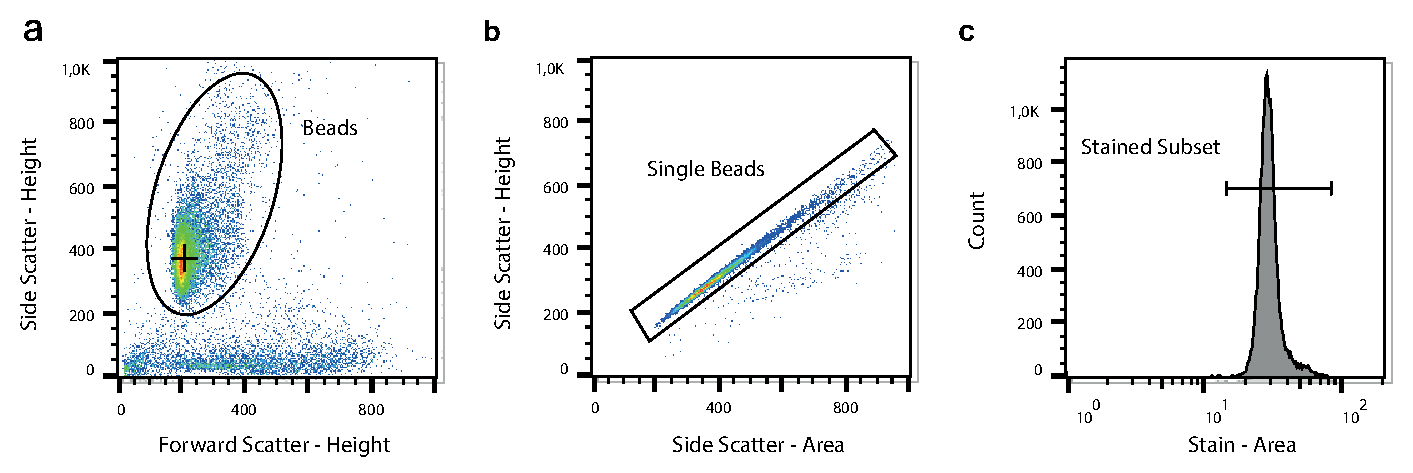
\includegraphics[width=\linewidth] {Ressources/GatingStrategy/GatingStrategy-Layout_with_margin.eps}
	\capption{Gating Strategy for Biotinylated Beads}{\textbf{a}, In the forward-side-scatter plot, the general bead population with high side scatter is selected from the background. \textbf{b}, Single beads are differentiated by their sphericity, their ratio of height:area in the side scatter. Points on the line through the origin are spherical. \textbf{c}, The stained subset in the respective color is now selected and the \gls{mfi} as well as the \gls{cv} is computed.}
	\label{fig:gatingstrategy-layout}
\end{figure}

Characterization of any surface modification was done via fluorescence-flow cytometry or -microscopy. \SIrange{30000}{60000}{beads} were diluted to \SI{20}{\micro\liter} and incubated with \SI{100}{\nano\gram} streptavidin-atto488 (49937, Sigma Aldrich) or Anti-Biotin-PE (\todo{which anti-biotin exacly} Miltenyi) for \SI{30}{\minute} at \SI{8}{\degreeCelsius} in a shaker. The beads were then diluted to a final volume of \SI{100}{\micro\liter}, transferred to a 96-well plate (TPP) and measured in the autosampler of a flow cytometer (MACS Quant Analyzer 10, Miltenyi). Following parameters were held constant over all measurements: \textit{Flow Rate:} High, \textit{Mix Sample:} Strong, \textit{Mode:} Standard, \textit{Uptake/Sample Volume:} \SI{100}{\micro\liter}. The photmultiplier voltages of forward and side scatter were lowered in most experiments by \SI{10}{\volt} and \SI{120}{\volt} respectively due to the homogeneous and reflective nature of the particles.
Data analysis was performed by FlowJo (10.6.2, Becton Dickinson) after a gating strategy which is depicted in Fig. \ref{fig:gatingstrategy-layout}. 
For fluorescence microscopy, the beads were stained with streptavidin-atto488 after the same procedure and imaged statically on a covered microscope slide at an exposure time of \SI{>100000}{\micro\second} and a gain \num{>15}. Images were then processed by Fiji. Im both measurements, the resulting data was plotted in Origin (2020b, OriginLab).



\subsubsection{Coating of Biofunctionalized Non-Magnetic Beads with Magnetic Nanoparticles}
The biotinylated, non-magnetic microbeads (Table \ref{tab:particles}) were coated covalently with different \glspl{mnp} in order to establish a bead-side titration of binding sites. Therefore, \SI{5}{\milli\gram\per\milli\liter} biotinylated beads in \gls{pbst} were equilibrated for \SI{10}{\minute} and mixed with \SI{7.5}{\micro\gram} BNF-dextran-redF-streptavidin / nanomag-D-spio, \SI{6}{\micro\gram} of SV0050 or \SI{10}{\micro\gram} Dynabeads C1 over night on a shaker. Afterwards, the supernatants were exchanged twice by careful centrifugation to avoid sedimentation of the nanoparticles.


